This section details the web interface layer and the three subsystems that it encompasses. The web interface layer includes the login, feedback and arrow key interface subsystems.

\subsection{Layer Hardware}
The Web Interface layer runs as a web server ontop of a Raspberry Pi Zero. The Raspberry Pi Zero runs off Raspbian OS which is a flavor of Debian Jessie. 

\subsection{Layer Operating System}
This layer relies on Raspbian OS which is a flavor of Debian Jessie.

\subsection{Layer Software Dependencies}
The Web Interface relies on jQuery, HTML, CSS, Python, Python Flask, and the GPIO Zero Python library.

\subsection{Login Subsystem}
The login sybststen will receive internet access from the black box system and be the first interface that the user will arrive at. The user will be required to access the system using a password or username stored in a database on the Raspberry Pi.

\begin{figure}[h!]
	\centering
 	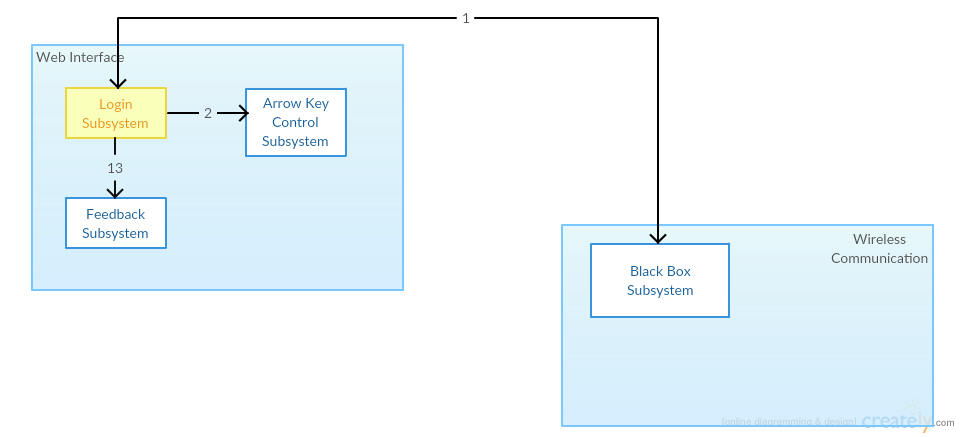
\includegraphics[width=0.60\textwidth]{images/ADSdiagrams/loginsubsystem.png}
 \caption{Diagram of the Login Subsystem}
\end{figure}

\subsubsection{Login Subsystem Software Dependencies}
The Login Subsystem relies on jQuery, HTML, CSS, Python, and Python Flask.

\subsubsection{Login Subsystem Programming Languages}
Javascript, HTML, CSS, and Python were used to create this subsystem.

\subsubsection{Login Subsystem Data Structures}
The Login Subsystem formats all requests to the server in a JSON format to send to the server.


\subsection{Arrow Key Control Subsystem}
The arrow key control subsystem is reached after a successful validation from the login subsystem and provides the ability to pan and tilt the camera.

\begin{figure}[h!]
	\centering
 	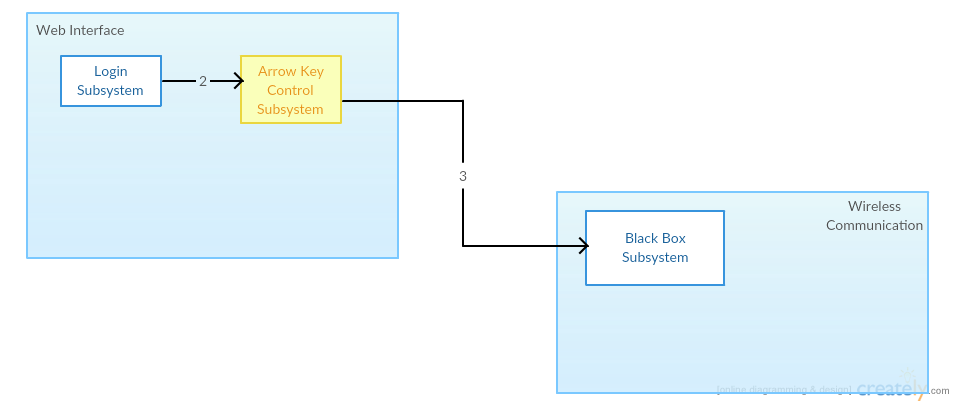
\includegraphics[width=0.60\textwidth]{images/ADSdiagrams/arrowkeycontrolsubsystem.png}
 \caption{Diagram of the arrow key control subsystem}
\end{figure}

\subsubsection{Arrow Key Control Subsystem Software Dependencies}
The Arrow Key Control Subsystem relies on jQuery, HTML, CSS, Python, Python Flask, and the GPIO Zero Python Library. 

\subsubsection{Arrow Key Control Subsystem Programming Languages}
Javascript, HTML, CSS, and Python were used to create this subsystem.

\subsubsection{Arrow Key Control Subsystem Data Structures}
The Login Subsystem formats all requests to the server in a JSON format to send to the server.

\subsection{Feedback Subsystem Subsystem}
The feedback subsystem is responsible for relaying the camera feed back to the user once they have been successfully validated by the login subsystem.

\begin{figure}[h!]
	\centering
 	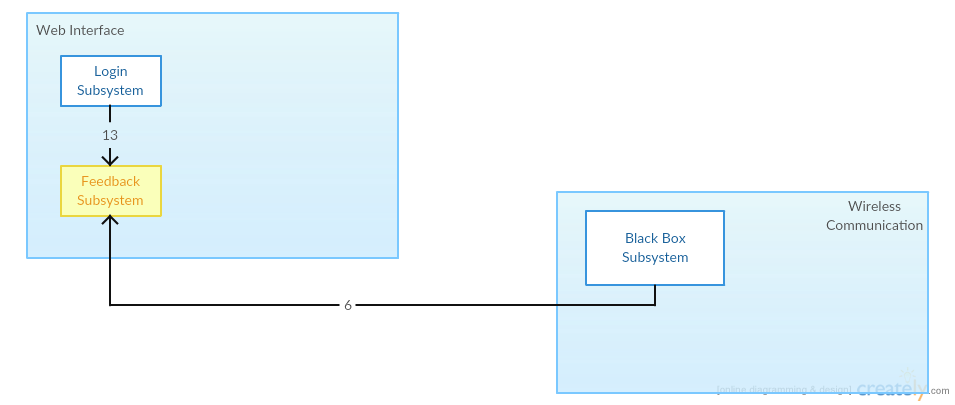
\includegraphics[width=0.60\textwidth]{images/ADSdiagrams/feedbacksubsystem.png}
 \caption{Diagram of the feedback subsystem}
\end{figure}

\subsubsection{Feedback Subsystem Software Dependencies}
The Feedback Subsytem relies on UV4l to provide the camera stream back to the user. 

\subsubsection{Feedback Subsystem Data Structures}
The Feeback Subsystem formats the camera stream as an mjpeg stream to send back to the user.
